\scanpage{253}
% Manuscript upside down in the scan; references follow the upright writing.
\[
J\subset A
\]
$H^*(X,J)^{\deleted{\unsure{*}}}$ à p.d.
% A long diagonal stroke begins to the left of the following presentation.
\[
\begin{aligned}
A\{(X_i)_{i\in I},(Y_i)_{i\in I}\}/\bigl(&\textstyle\sum X_i-\pi,\sum Y_i-\omega,\sum dX_i,\\
&\textstyle\sum dY_i\bigr)
\end{aligned}
\]
\[
\overset{\unsure{\sim|-|\rightarrow}}{\deleted{A}\quad A^{(I)}}
\]
\figure{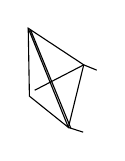
\begin{tikzpicture}[scale=.75]\draw (0,1.6)--(.94,.98)--(.68,-.08)--(.02,.45)--cycle;\draw (0,1.6)--(.68,-.08) (.04,1.57)--(.72,-.09) (.11,.55)--(.94,.98); \draw (.94,.98)--(1.16,.89) (.68,-.08)--(.93,-.16);\end{tikzpicture}}
\deleted{\[
\begin{aligned}
&\Gamma^*_{(A,\pi)}(A^I\otimes_A J)\\
&X_{\unsure{1|i}}\otimes\pi,\ X_{\unsure{2}}\otimes\pi,\ -,\ X_{\unsure{m|n}}\otimes\pi\\
&\textstyle\sum X_i\otimes\pi-\pi\\
&\deleted{J^I/J}\\
&\Gamma^*_{(A,J)}(J^I)/\delta J\\
&\delta\pi=\deleted{\unsure{\pi}}-\pi+\pi
\end{aligned}
\]}
$\unsure{K|L|\Gamma}_A^*.$
\deleted{\[
A\bigl\{(X_i)_{i\in I}\inserted{dX_i}\bigr\}/\bigl(\sum_{\unsure{I}}\pi X_i-\pi\,;\ \pi\sum dX_i\bigr\}
\]}
\[
\Gamma_A^{*+}J\longrightarrow J
\]
\[
H^*(X,\Gamma^{\alpha+}J)\longrightarrow H^\alpha(X,J)
\]
\deleted{\diagram{\begin{tikzcd}[ampersand replacement=\&]
\&\& H^{\unsure{2\alpha|2i\alpha}}(X,\operatorname{Sym}^{\alpha}M)\\
H^{2i}(X,M)\arrow[r,"\gamma^\alpha"] \& H^{2i\alpha}(X,\Gamma^\alpha M)\arrow[ur] \&
\end{tikzcd}}
\[
H^{2i}(X,J)\longrightarrow H^{2i\alpha}(X,\Gamma^\alpha J)\longrightarrow H^{2i\alpha}(X,J)
\]}
\diagram{\begin{tikzcd}[ampersand replacement=\&]
A\arrow[r,"2i"]\arrow[dr,"2i\alpha"'] \& M\\
\&\Gamma^\alpha M
\end{tikzcd}}
\diagram{\begin{tikzcd}[ampersand replacement=\&]
\Gamma^i M\arrow[d,shift right] \& x^{(i)}\arrow[d,mapsto]\& \substack{i!x^{(i)}\\ \Vert\\ x^i}\\
\operatorname{Sym}^i(M)\arrow[u,shift right]\&x^i\&\unsure{x}\arrow[u]
\end{tikzcd}}
% archive sheet number: 252
